\documentclass[11pt, letterpaper,titlepage]{article}

% --- Essential Packages ---
\usepackage[utf8]{inputenc}
\usepackage[margin=1in]{geometry}
\usepackage{fancyhdr} % For custom headers and footers
\usepackage{graphicx}
\usepackage{amsfonts}

\usepackage{amsmath}
\usepackage{float}

\usepackage{hyperref}
\usepackage{setspace}

\usepackage{ragged2e}
\usepackage{parskip}

\usepackage{booktabs}
% --- Header/Footer Configuration ---
\pagestyle{fancy}
\fancyhf{} % Clear all default header and footer settings
\fancyhead[L]{DIGITALLY CONTROLLED ANALOG MIXER} % Left header text
\fancyhead[C]{} % Center header text (empty)
\fancyhead[R]{\thepage} % Right header (page number)
\renewcommand{\headrulewidth}{0.4pt} % Line below header
\linespread{1.2}





\begin{document}
\begin{titlepage}
    \centering
    \vspace*{0cm}
    
    {\huge \textbf{Analog Mixing Console with Digital Control\\ \vspace{0.5cm}and Automated Signal Path Configuration}} \\[1cm]
    
    \vspace{0.5cm}
    
    {\huge Capstone Project Report}
    
    \vspace{5cm}
    




    
    {\Large \textbf{Skylar Denno}}
    
    \vspace{0.3cm}
    
    {\Large \textbf{Darya Petrova}}
    
        \vspace{0.3cm}
    
    {\Large \textbf{Evan Forcucci}}
    
        \vspace{0.3cm}
    
    {\Large \textbf{Xinhao Chen}}
    
        \vspace{0.3cm}
    
    {\Large \textbf{Luke Garrity}}
    
        \vspace{0.3cm}
    
    {\Large \textbf{Daniel Salas}}
    

    
    \vspace{0.5cm}
    
        {\large \textbf{Advisor: }Milad Siami \textbf{[Team \#2]}}
    
        \vspace{1.3cm}

    
        {\LARGE \textbf{Northeastern University}} \\
        
    Department of Electrical and Computer Engineering \\
    \vspace{1cm}
    
    
    \today

\end{titlepage}
\setlength{\parindent}{6pt}

\justify

\tableofcontents
\newpage

\section{Introduction}
\subsection{Background}
\subsection{Problem Statement}
\subsection{Scope and Design Goals}

\newpage

\section{Analog Design}

\subsection{Analog Systems Overview}



\subsection{Voltage Controlled Amplifiers}
\label{sec:vca}
% ----------------------------------------------------------------------------
% [PROSE] Opening -- sketch:
%   - Every gain in the console is set by a DC control voltage from the digital
%     side; the audio never passes through a digital stage.
%   - Pan/fader module used to introduce the basics: two identical VCAs, one
%     control voltage each, so the VCA and its temperature behavior can be
%     shown without extra circuitry. EQ, input and compressor modules reuse this.
%   - Part: THAT2180A (Blackmer log-antilog cell): dB-linear control,
%     >120 dB dynamic range, 0.005 % THD typ., pre-trimmed. [cite datasheet]
%   - One sentence on the module path (input buffer -> insert switching ->
%     two VCAs -> I/V -> balanced bus drivers), point to Fig.~\ref{fig:vca-stage}.
% ----------------------------------------------------------------------------
The most fundamental part of an audio mixer is control of each individual channels' gain before summing to the final stereo signal. To implement gain control that can be remote controlled by a voltage, voltage controlled amplifiers (VCAs) were used. Two VCAs were actually used on every channel. Since we aim to build a stereo mixer, the two VCAs feed the left and right summing channel of the mix bus, respectively. Each channel's two VCAs may be given different gain control voltages (CVs) to pan the channel's audio in the stereo field. For example, if a channel's left VCA had a CV to attenuate by -90dB (basically muted) and the right VCA had the CV to add 6dB of gain, that channel's audio would sound like it was coming from the right speaker after summing. To implement the regular fader behavior, which changes the gain of the left and right side together, both the left and right control voltages would be scaled together to change gain equally in both channels.

The specific VCA we picked for this purpose was the THAT 2180 from the Massachusetts-based THAT Corporation. It is the industry standard VCA for high fidelity audio performance. This is due to its total harmonic distortion (THD) of just 0.005\% (for the 'A' grade 2180s), which is extremely low for a VCA. Additionally, it uses a Blackmer gain cell, which has a logarithmic gain curve, allowing control voltage and decibel gain to coincide linearly. Unfortunately, in September 2026, halfway through the design of the project, THAT Corporation announced it was discontinuing its legendary 2180 series, sending shockwaves through the audio electronics community. Frantically, we bought 32 of the 'A' grade THAT 2180s to use for this purpose, but the rest of the analog systems use clones of the THAT 2180 (Alfa RPAR AS2180, which from our tests, seems to have nearly as good performance as the genuine 'A' grade 2180s) or the SSI2164 VCA.


\begin{figure}[H]
    \centering
    % \includegraphics[width=0.8\textwidth]{figures/vca_stage.pdf}
    \fbox{\parbox[c][4.5cm][c]{0.8\textwidth}{\centering
        Placeholder: one VCA channel --- $C_\text{in}$, $R_\text{in}$, THAT2180A,
        I/V converter ($R_f \parallel C_f$), control-port snubber, $R_\text{SET}$}}
    \caption{One channel of the pan/fader VCA stage.}
    \label{fig:vca-stage}
\end{figure}

\paragraph{Current-mode operation.}
% [PROSE] sketch:
%   - Current in, current out: pins 1 and 8 sit at virtual ground.
%   - R_in turns the input voltage into a current; an op-amp I/V converter turns
%     the output current back into a voltage. Overall path is non-inverting.
%   - With R_f = R_in the stage is unity gain when the cell is at 0 dB.
\begin{equation}
    I_\text{in} = \frac{V_\text{in}}{R_\text{in}}, \qquad
    I_\text{out} = A_I\, I_\text{in}, \qquad
    V_\text{out} = R_f\, I_\text{out}
    \quad\Longrightarrow\quad
    \frac{V_\text{out}}{V_\text{in}} = \frac{R_f}{R_\text{in}}\,A_I
    \label{eq:vca-transfer}
\end{equation}

\paragraph{Exponential gain control.}
% [PROSE] sketch:
%   - The cell logs the input current across matched junctions, adds the control
%     voltage, and antilogs it back. [cite THAT DN128 / Hebert, AES 1995]
%   - Gain is exponential in the control voltage, i.e. linear in dB.
%   - kappa comes from kT/q; datasheet value 6.1 mV/dB at a die temperature of
%     about 35 C.
%   - E_C+ carries the fader/pan CV here; E_C- is grounded (the compressor CV
%     enters there in a later module).
\begin{equation}
    \begin{gathered}
    A_I = \exp\!\left(\frac{q\,(E_{C+}-E_{C-})}{2kT}\right)
    \quad\Longrightarrow\quad
    G_\text{dB} = 20\log_{10}A_I = \frac{E_{C+}-E_{C-}}{\kappa(T)}, \\
    \kappa(T) = \frac{\ln 10}{10}\,\frac{kT}{q} \approx 6.1\ \mathrm{mV/dB}
    \end{gathered}
    \label{eq:vca-law}
\end{equation}

\paragraph{Temperature sensitivity.}
% [PROSE] sketch:
%   - kappa is proportional to absolute temperature (PTAT), so the dB gain scales
%     by T0/T: a span error that pivots about 0 dB.
%   - Example: -20 dB setting, +20 C warm-up -> about 1.3 dB error. This is what
%     Section~\ref{sec:cv-buffer} compensates.
\begin{equation}
    G_\text{dB}(T) = G_\text{dB}(T_0)\,\frac{T_0}{T}
    \quad\Longrightarrow\quad
    \frac{\Delta G_\text{dB}}{G_\text{dB}} \approx -\frac{\Delta T}{T_0} \approx -0.33\,\%/\mathrm{K}
    \label{eq:vca-tempco}
\end{equation}

\paragraph{Operating point.}
% [PROSE] sketch:
%   - Pin 5 is not a supply: R_SET sets the cell current (pin sits about four
%     Vbe below ground). Datasheet rule: I_SET covers the peak signal currents
%     plus 570 uA of bias. Worst case 0 dB with a 14 V peak: 0.70 mA in and out.
%   - Control port must be driven from well under 50 ohm: base currents are
%     signal-related, and 10 uV of audio at the port already gives 0.01 % THD.
%     Hence op-amp drive plus a shunt RC snubber at the pin.
%   - Remaining choices in Table~\ref{tab:vca-op}.
\begin{equation}
    I_\text{SET} = \frac{V_\text{pin5}-V_{EE}}{R_\text{SET}}
    = \frac{-2.85\,\mathrm{V}+15\,\mathrm{V}}{5.1\,\mathrm{k}\Omega} = 2.38\,\mathrm{mA}
    \;\geq\; \hat I_\text{in} + \hat I_\text{out} + 570\,\mu\mathrm{A} = 1.97\,\mathrm{mA}
    \label{eq:iset}
\end{equation}

\begin{table}[H]
    \centering
    \begin{tabular}{@{}lll@{}}
        \toprule
        Component & Value & Purpose \\
        \midrule
        $R_\text{in}$, $R_f$ & $20\,\mathrm{k}\Omega$ & unity gain at 0 dB; datasheet noise/THD point \\
        $C_\text{in}$ & $10\,\mu\mathrm{F}$ bipolar & $f_c = 1/(2\pi R_\text{in} C_\text{in}) = 0.8$ Hz; blocks DC \\
        $C_f$ & $22\,\mathrm{pF}$ & cancels 15 pF at pin 8 (I/V stability) \\
        $R_\text{SET}$ & $5.1\,\mathrm{k}\Omega$ & $I_\text{SET} = 2.38$ mA, Eq.~\eqref{eq:iset} \\
        Port snubber & $100\,\Omega$ + $2.2\,\mathrm{nF}$ to ground & damps inductive op-amp output \\
        Sym (pin 4) & open & keeps factory THD trim \\
        \bottomrule
    \end{tabular}
    \caption{THAT2180A operating point.}
    \label{tab:vca-op}
\end{table}

\paragraph{Pan and fader law.}
% [PROSE] sketch:
%   - Constant-power pan: the sum of squares is constant, so a source keeps its
%     loudness across the stereo field; -3.01 dB per side at centre.
%   - Because the VCA is dB-linear, fader and pan simply add in the control
%     domain: no multiplier, one CV per channel, computed in firmware.
\begin{gather}
    g_L = G\cos\!\left(\tfrac{\pi\theta}{2}\right), \qquad
    g_R = G\sin\!\left(\tfrac{\pi\theta}{2}\right), \qquad
    g_L^2 + g_R^2 = G^2, \qquad \theta \in [0,1]
    \label{eq:panlaw}\\
    G_{\text{dB},L} = 20\log_{10}G + 20\log_{10}\cos\!\left(\tfrac{\pi\theta}{2}\right), \qquad
    G_{\text{dB},R} = 20\log_{10}G + 20\log_{10}\sin\!\left(\tfrac{\pi\theta}{2}\right)
    \label{eq:panlaw-db}
\end{gather}

\subsection{Control Voltage Buffering and Temperature Drift Compensation}
\label{sec:cv-buffer}
% ----------------------------------------------------------------------------
% [PROSE] Opening -- sketch:
%   - One op-amp stage per channel has four jobs: (1) map the DAC range onto the
%     VCA's useful control range, (2) drive the control port from a low
%     impedance, (3) filter DAC steps and noise (ripple on E_C modulates the
%     audio), (4) cancel the PTAT drift of Eq.~\eqref{eq:vca-tempco}.
%   - Topology: inverting multiple-feedback (MFB) low-pass fed by a small
%     network -- DAC current, an offset current from a -2.5 V reference, and
%     an NTC thermistor. Fig.~\ref{fig:cv-buffer}, values in
%     Table~\ref{tab:cv-values}.
%   - Why MFB: inverting (the sign needed), good rejection far above the
%     corner, scaling and filtering in one stage.
% ----------------------------------------------------------------------------

\begin{figure}[H]
    \centering
    % \includegraphics[width=0.8\textwidth]{figures/cv_buffer.pdf}
    \fbox{\parbox[c][4.5cm][c]{0.8\textwidth}{\centering
        Placeholder: CV buffer --- DAC input, $R_\text{cv}$ + trim,
        $R_\text{off}$ to $-2.5$ V, $R_p \parallel R_\text{NTC}$,
        MFB ($R_2$, $R_3$, $C_1$, $C_2$), OPA2197, snubber at $E_{C+}$}}
    \caption{Control voltage buffer for one VCA.}
    \label{fig:cv-buffer}
\end{figure}

\begin{figure}[H]
\centering
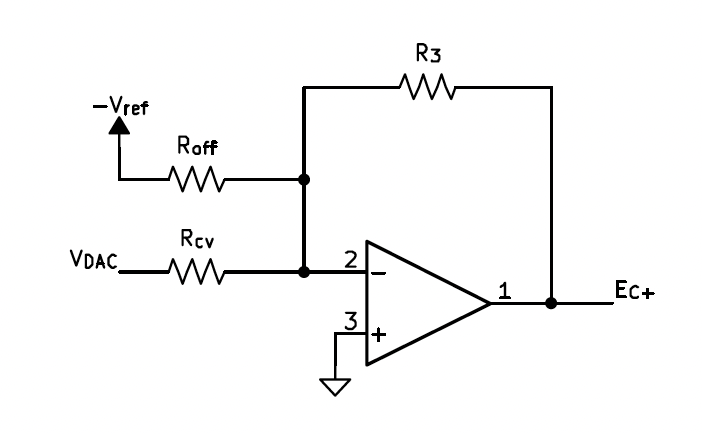
\includegraphics[width=0.5\textwidth]{images/cv_buffer_1_scaler} 
\caption{TEST}
\end{figure}

\begin{figure}[H]
\centering
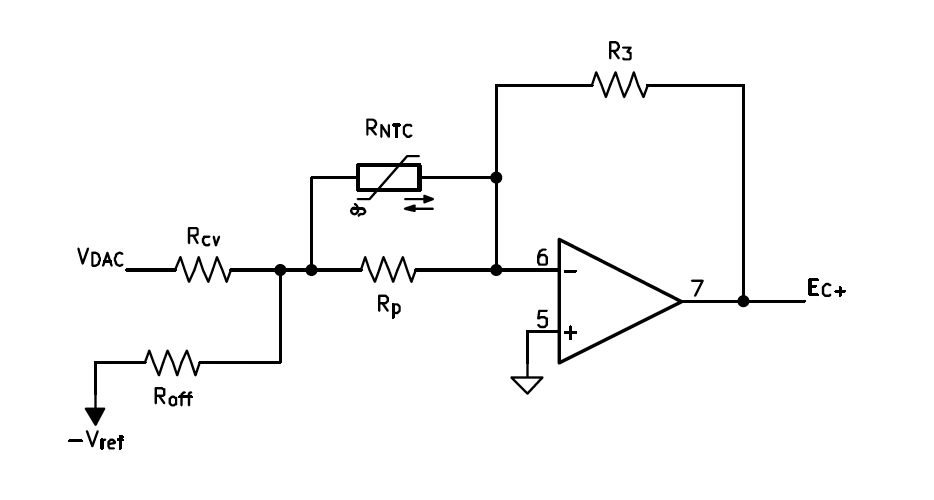
\includegraphics[width=0.5\textwidth]{images/cv_buffer_2_tempcomp} 
\caption{TEST}
\end{figure}

\begin{figure}[H]
\centering
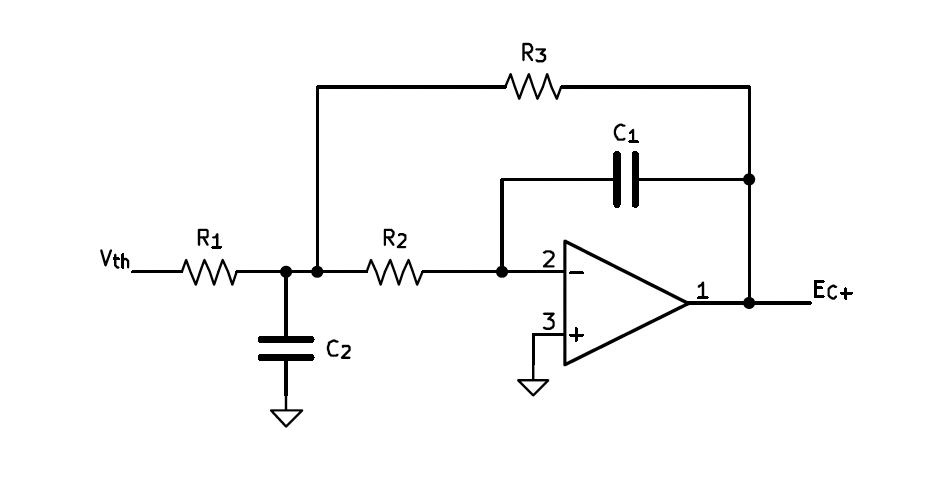
\includegraphics[width=0.5\textwidth]{images/cv_buffer_3_multifb} 
\caption{TEST}
\end{figure}

\begin{figure}[H]
\centering
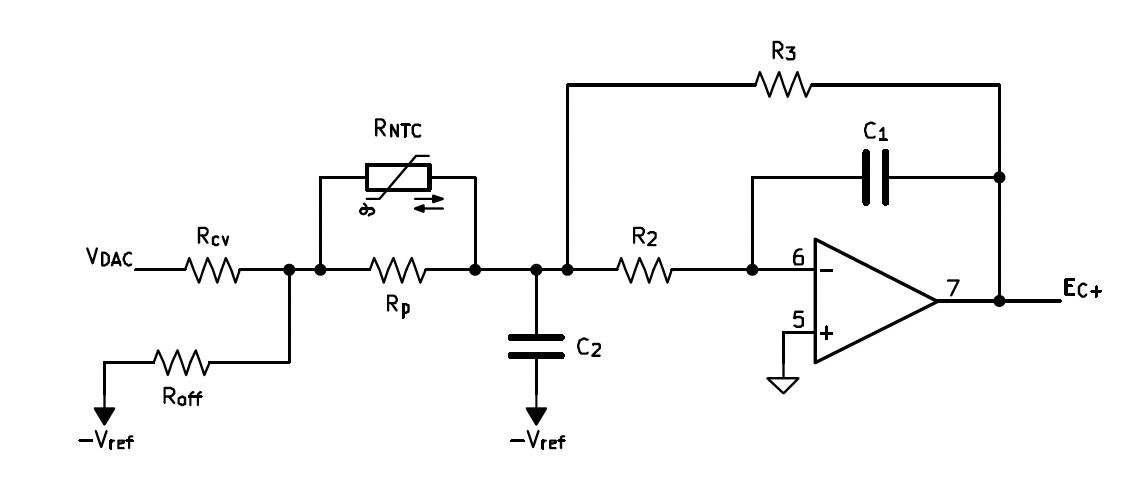
\includegraphics[width=0.5\textwidth]{images/cv_buffer_4_full} 
\caption{TEST}
\end{figure}

\begin{figure}[H]
\centering
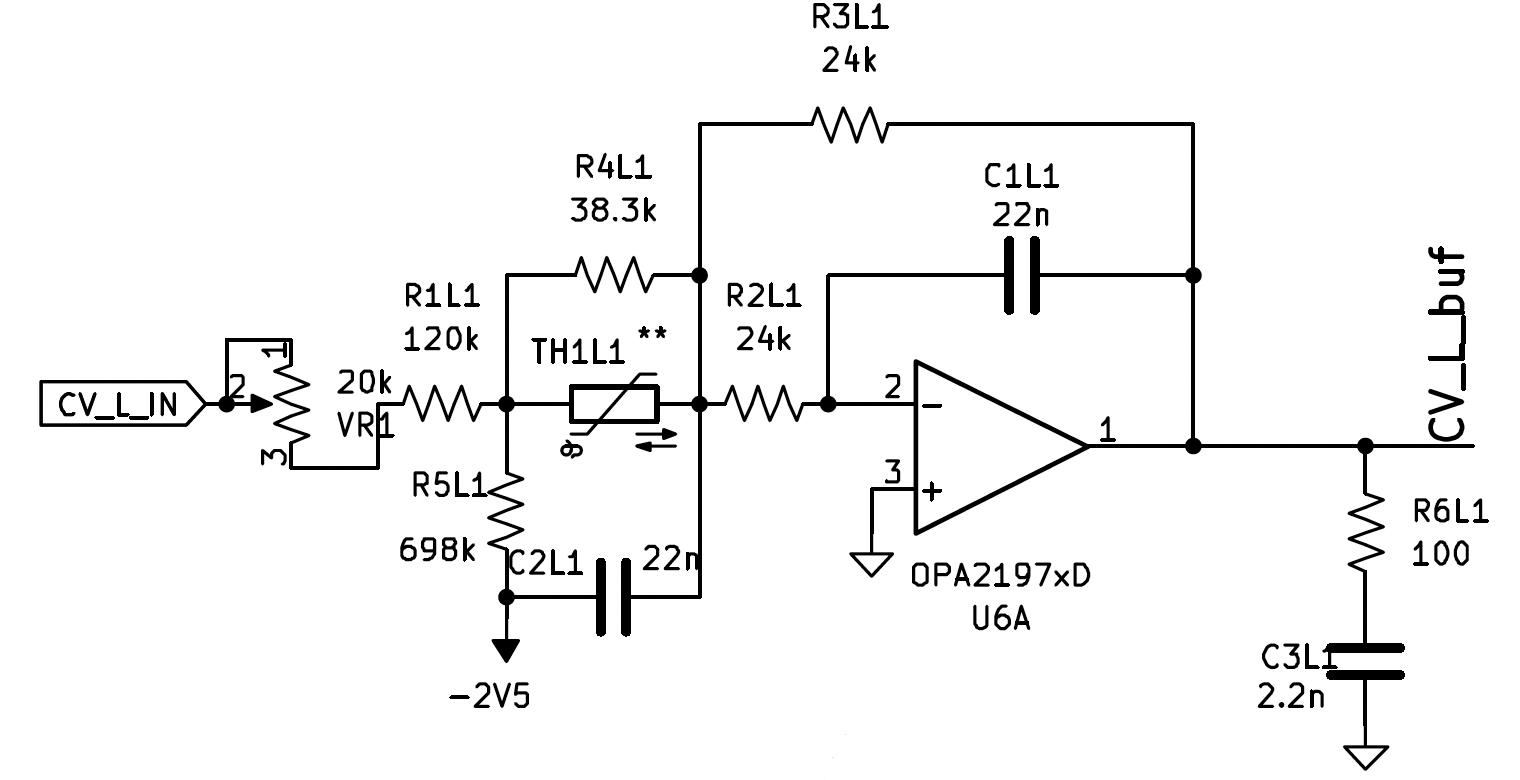
\includegraphics[width=0.7\textwidth]{images/cv_buffer_5_final} 
\caption{The trim potentiometer on the left is ONLY to calibrate temperature scaling during assembly, and it is not accessible to the end user.}
\end{figure}

\begin{table}[H]
    \centering
    \begin{tabular}{@{}lll@{}}
        \toprule
        Component & Value & Role \\
        \midrule
        $R_\text{cv}$ & $120\,\mathrm{k}\Omega$ + $20\,\mathrm{k}\Omega$ trim ($133\,\mathrm{k}\Omega$ nom.) & DAC voltage to current; span trim \\
        $R_\text{off}$ & $698\,\mathrm{k}\Omega$ & offset current \\
        $R_p \parallel R_\text{NTC}$ & $38.3\,\mathrm{k}\Omega \parallel 47\,\mathrm{k}\Omega$ ($B = 4090$ K) & temperature compensation \\
        $R_2 = R_3$ & $24\,\mathrm{k}\Omega$ & filter and DC gain \\
        $C_1 = C_2$ & $22\,\mathrm{nF}$ film & filter \\
        $V_\text{ref}$ & 2.5 V (ADR5041 at $-2.5$ V, $222\,\mu$A bias) & offset reference \\
        Op-amp & OPA2197 & low offset and noise \\
        \bottomrule
    \end{tabular}
    \caption{CV buffer component values (one channel).}
    \label{tab:cv-values}
\end{table}

\paragraph{DAC.}
% [PROSE] sketch:
%   - MCP4728, internal 2.048 V reference at gain 2: 1 mV per code, and the
%     scale no longer depends on the 5 V rail.
\begin{equation}
    V_\text{DAC} = \frac{2V_\text{REF}}{4096}\,n = n \times 1\,\mathrm{mV}, \qquad
    V_\text{REF} = 2.048\,\mathrm{V}, \quad n \in \{0,\dots,4095\}
    \label{eq:dac}
\end{equation}

\paragraph{DC transfer.}
% [PROSE] sketch:
%   - Replace the DAC and offset branches by their Thevenin equivalent; Z_t is
%     in series, so the MFB sees one input resistor R_1.
%   - The node between Z_t and the MFB stays at 0 V DC (C_1 blocks DC and R_2
%     returns to the virtual ground), so the DC gain is simply -R_3/R_1.
%   - D is the fraction of the source current that reaches the MFB -- the
%     quantity the thermistor adjusts.
\begin{gather}
    R_\text{th} = R_\text{cv} \parallel R_\text{off}, \qquad
    V_\text{th} = R_\text{th}\left(\frac{V_\text{DAC}}{R_\text{cv}} - \frac{V_\text{ref}}{R_\text{off}}\right), \qquad
    Z_t = R_p \parallel R_\text{NTC}(T), \qquad
    R_1 = R_\text{th} + Z_t
    \label{eq:thevenin}\\
    E_{C+} = -\frac{R_3}{R_1}\,V_\text{th}
    = -R_3\,D\left(\frac{V_\text{DAC}}{R_\text{cv}} - \frac{V_\text{ref}}{R_\text{off}}\right), \qquad
    D = \frac{R_\text{th}}{R_\text{th}+Z_t}
    \label{eq:cv-dc}
\end{gather}
% [PROSE] sketch: with Table~\ref{tab:cv-values} at 25 C, Z_t = 21.1 k and
%   D = 0.841; give the resulting map.
\begin{equation}
    E_{C+} = 72.3\,\mathrm{mV} - 0.1518\,V_\text{DAC}
    \quad\Longrightarrow\quad
    G_\text{dB} = 11.9\,\mathrm{dB} - 24.9\,\tfrac{\mathrm{dB}}{\mathrm{V}}\,V_\text{DAC}
    \label{eq:cv-numeric}
\end{equation}

\paragraph{Code mapping.}
% [PROSE] sketch:
%   - Firmware applies the pan law (Eq.~\eqref{eq:panlaw-db}), then inverts
%     Eq.~\eqref{eq:cv-numeric} per channel. 0.025 dB per code.
%   - 0 V gives +12 dB and full scale about -90 dB, used as mute; the DAC's
%     power-up code is stored as 4095 so the board starts silent.
\begin{equation}
    n = \frac{72.3\,\mathrm{mV} - \kappa\,G_\text{dB}}{0.1518 \times 1\,\mathrm{mV}}
    \label{eq:code}
\end{equation}

\begin{table}[H]
    \centering
    \begin{tabular}{@{}lccccccc@{}}
        \toprule
        $G_\text{dB}$ & $+11.9$ & $+6$ & $0$ & $-3.01$ & $-20$ & $-70$ & $-90$ \\
        \midrule
        $n$ & 0 & 235 & 476 & 597 & 1280 & 3290 & 4095 \\
        \bottomrule
    \end{tabular}
    \caption{Example codes from Eq.~\eqref{eq:code} (nominal, before calibration).}
    \label{tab:codes}
\end{table}

\paragraph{Filtering.}
% [PROSE] sketch:
%   - Second-order low-pass smooths the 1 mV steps (zipper noise) and removes
%     digital noise before it reaches the control port.
%   - Q < 0.5 on purpose: no overshoot, since an overshooting CV is an
%     overshooting gain.
%   - Attenuation: -22 dB at 1 kHz, -40 dB at 3 kHz, -61 dB at 10 kHz.
%   - C_2 returns to the -2.5 V reference, which is an AC ground.
\begin{gather}
    \frac{E_{C+}(s)}{V_\text{th}(s)} = -\frac{R_3}{R_1}\,
    \frac{1}{1 + sC_1\!\left(R_2 + R_3 + \frac{R_2R_3}{R_1}\right) + s^2R_2R_3C_1C_2}
    \label{eq:mfb}\\
    f_0 = \frac{1}{2\pi\sqrt{R_2R_3C_1C_2}} = 301\,\mathrm{Hz}, \qquad
    Q = \frac{\sqrt{R_2R_3C_1C_2}}{C_1\left(R_2 + R_3 + R_2R_3/R_1\right)} = 0.46
    \label{eq:mfb-f0q}
\end{gather}

\paragraph{Temperature compensation.}
% [PROSE] sketch:
%   - From Eq.~\eqref{eq:vca-law}: to hold a dB setting, the control voltage
%     must itself grow in proportion to absolute temperature.
%   - E_C+ is proportional to D, and D depends on temperature only through Z_t,
%     so it is enough to make D PTAT (Eq.~\eqref{eq:dD}).
%   - The NTC is bent against the 2180 package so it follows the die; the pad
%     R_p flattens the NTC's exponential so the slope holds over a useful range.
%   - Two free parameters (R_p, R_th): set the slope at T_0 with
%     Eq.~\eqref{eq:comp-cond}, then check the residual over the range.
\begin{gather}
    E_{C+}(T) = E_{C+}(T_0)\,\frac{T}{T_0}
    \quad\Longrightarrow\quad
    \frac{1}{E_{C+}}\frac{dE_{C+}}{dT} = \frac{1}{T_0} \approx 0.33\,\%/\mathrm{K}
    \label{eq:ptat-req}\\
    \frac{1}{D}\frac{dD}{dT} = -(1-D)\,\frac{1}{Z_t}\frac{dZ_t}{dT}
    \label{eq:dD}\\
    R_\text{NTC}(T) = R_{25}\,e^{B\left(\frac{1}{T}-\frac{1}{T_{25}}\right)}, \qquad
    \frac{dR_\text{NTC}}{dT} = -\frac{B}{T^2}R_\text{NTC}, \qquad
    \frac{dZ_t}{dT} = \left(\frac{R_p}{R_p+R_\text{NTC}}\right)^{2}\frac{dR_\text{NTC}}{dT}
    \label{eq:ntc}\\
    (1-D)\left|\frac{1}{Z_t}\frac{dZ_t}{dT}\right|_{T_0} = \frac{1}{T_0}
    \label{eq:comp-cond}
\end{gather}
% [PROSE] sketch: numbers at T_0 = 25 C below. Result: residual scale error
%   0.39 % over 10--40 C (0.08 dB at -20 dB) against 1.3 dB uncompensated.
%   Optional: plot of compensated vs uncompensated error over temperature.
\begin{align}
    \left.\frac{dR_\text{NTC}}{dT}\right|_{T_0} &= -2.16\,\mathrm{k}\Omega/\mathrm{K}, &
    \frac{1}{Z_t}\frac{dZ_t}{dT} &= \frac{-436\,\Omega/\mathrm{K}}{21.1\,\mathrm{k}\Omega} = -2.07\,\%/\mathrm{K},
    \nonumber\\
    1-D &= 0.159, &
    \frac{1}{D}\frac{dD}{dT} &= 0.159 \times 2.07\,\%/\mathrm{K} = 0.33\,\%/\mathrm{K}
    \label{eq:comp-numbers}
\end{align}

\paragraph{Calibration.}
% [PROSE] sketch:
%   - Remaining static errors: resistor tolerances, DAC reference (+/-2 %), DAC
%     zero offset.
%   - Span: the 20 k trimmer in series with R_cv (120--140 k, +/-7.7 %) sets the
%     slope; it sits in the input leg so it barely affects the filter.
%   - Zero: in firmware. Measure the gain at two codes after warm-up and
%     interpolate, since the law is linear in dB.
\begin{equation}
    n(G_\text{dB}) = n_a + \left(G_\text{dB} - G_a\right)\frac{n_b - n_a}{G_b - G_a}
    \label{eq:cal}
\end{equation}

\subsection{Channel Routing and Auxiliary Buses}
\subsection{Voltage Controlled State Variable Filters and EQ Circuit}
\subsection{Input Circuitry and Preamplifier}
\subsection{Hybrid Digital/Analog Dynamic Range Compressor}
\subsection{Mix Bus and Master Section}
\subsection{Channel Insert Routing Matrix}
\subsection{PCB Design Notes}

\newpage
\section{Digital Systems}

\subsection{Digital Systems Overview}
\subsection{I2C Buses}
\subsubsection{I2C Communication Timings}
\subsubsection{Frames}
\subsubsection{Superframes}
\subsection{Control Panel Integration and Control Feedback}
\subsubsection{EC11 Rotary Encoders and Two-Bit Quadrature}
\subsubsection{Push-buttons and Debounce}
\subsubsection{MCP23017 GPIO Expanders}
\subsubsection{Shift-Register Based LED Scheme}
\subsection{LCD Displays}


\subsection{Saving of Console States}
\subsection{Communication Between Buckets and the Master Controller}
\subsection{USB Remote Control Computer Software}
\subsection{PCB Design Notes}

\newpage
\section{Testing and Results}
\subsection{Analog Performance Metrics}
\subsubsection{Linearity / Distortion}
\subsubsection{Noise}
\subsubsection{Temperature Drift Compensation}
\subsection{Digital System Bug Testing}

\newpage
\section{Financials}
\subsection{This Project's Budget and Bill of Materials}
\subsection{Exploration of Cost Reduction for Making a Commercial Product}



\end{document}